
\section{Line}
\label{section: line}

グラフがLineの場合,
グラフの全体(頂点と辺)をすべて実直線上におくことができる.
以降,頂点の名前$v_1, v_2, \ldots, v_n$はその位置を表す実数値も表すことにする.

まず,Lineの場合における順序保存運行という特別な運行を定義する.
運行$A$が順序保存であるとは,
$A$が定める巡査の位置$a_1, a_2, \ldots, a_m$が,
任意の時刻$t \in \Rset$において
$a_1(t) \leq a_2(t) \leq \cdots \leq a_m(t)$を満すことである.

Line上の任意の運行$A$は,$A$と同じ数の巡査でかつ警邏する点集合を保ったまま,順序保存運行$A'$に以下のように変換することができる.
%
まず,$A$が定める各巡査の運行を$a_1, a_2, \ldots, a_m$とする.
これに対し,
$a'_i (i \in \mathset{1, \ldots, m})$を
各時刻$t \in \Rset$において$a' _i(t)$が
$a_1(t), a_2(t), \ldots, a_m(t)$のうち$i$番目に小さいものとなるように定める.
すると,各$a' _i$は運行となっており,
$A' = (a' _i)_{ i \in \mathset{1,\ldots, m} }$とすると
$A'$の運行の軌跡の集合は$A$と等しいので,
(すなわち,任意の時刻$t \in \Rset$において$\mathset{a_1(t), \ldots, a_m(t)} = \mathset{a'_1(t), \ldots, a'_m(t)}$)
$A$で警邏していた点集合を$A'$も警邏している.
これにより順序保存運行$A'$が得られる.
%
順序保存運行$A'$は$A$において巡査がすれ違う時に代わりに互いの動きを交換することにより順序を保ったものとみなすことができる.

以上から,
巡査$m$人により警邏可能な任意の頂点集合$W$は,
巡査$m$人による或る順序保存運行$A'$によって警邏されることが分かる.




%%%%% section 2.1 %%%%%

\subsection{{\timelimit}がすべて等しい場合}
\label{subsec:LineUnaryTimelimit}




本節では次のことを示す.

\begin{theo}
    \label{theo:LineEqualTimelimit}
    グラフの形状がLineで{\timelimit}がすべて等しい場合,
    {\patrolling}は多項式時間で解くことができる.
\end{theo}

\red{この設定に関しては、やはりCollins et al.との関係を述べるべきではないか?}
この問題は,~~な場合については Collinsら~\ref{}の問題の特殊な場合として既に示されているが,
ここでは{\timelimit}がすべて等しいという条件のみでも成り立つことを示す.


以降では,
グラフの形状がLineで{\timelimit}がすべて等しい場合,
警邏可能な頂点集合のうち利得の和が最大となるものは
次に定義する個別往復運行という運行によって警邏可能であるということを示す.
Lineで{\timelimit}がすべて等しい場合に用いることができる
個別往復運行という戦略では
巡査の協力が不要になるため(補題\ref{lemm:LineEqualTimelimitIndependentInterval}),
{\timelimit}がすべて等しいという条件が問題を簡単にしているといえる.


\begin{defi}
    $V$を頂点集合,$Q$を各頂点の{\timelimit}とする.
    % $m$人の巡査による運行であって,
    % 各巡査が$V$のいずれかの頂点を左端とする長さ$Q/2$の区間を往復する運行を
    % $m$人の巡査による$V$上の個別往復運行と呼ぶ.
    各巡査が$V$のいずれかの頂点を左端とする長さ$Q/2$の区間を往復する運行を個別往復運行と呼ぶ.
    $m$人の巡査による運行$A$において各巡査が個別往復運行をしているとき,
    $A$を単に$m$人の巡査による個別往復運行と呼ぶ.
\end{defi}



まず次の補題を示す.

\begin{lemm}
    \label{lemm:RangeOfPatrollerOnLine}
    頂点$v_i$がある1人の巡査$s$により単独警備されているとき,
    {\timelimit}を$q_i$として,
    $s$は常に区間$[v_i - q_i/2, v_i + q_i/2]$にいる.
\end{lemm}

\begin{proof}[証明]
    \newcommand{\vout}{v_{\mathrm{out}}}
    この区間にない或る座標$\vout \notin [v_i - q_i/2, v_i + q_i/2]$を$s$が
    時刻$t_0$に訪問するとする.
    $\vout$と$v_i$の間の移動には
    少くとも時間$\lvert v_i - \vout \rvert > q _i / 2$を要するから,
    $s$は区間$[t_0 - q _i / 2, t_0 + q _i / 2]$に属する時刻に$v_i$を訪問できない.
    この区間の長さは$
        q_i
    $であるので,$s$が$v _i$を単独警備していることに反する.
\end{proof}



これにより次の補題が成り立つ.


\begin{lemm}
 \label{lemm:LineEqualTimelimitIndependentInterval}
    グラフの形状がLineで,頂点の{\timelimit}がすべて$Q$であるとする.
    頂点集合$W$が$m$人の巡査により警邏可能であるとする.
    このとき,
    $W$を警邏する$m$人の巡査による個別往復運行が存在する.
\end{lemm}


\begin{proof}[証明]

    \newcommand{\leftmostpoint}{b}  % v以外の記号
    \newcommand{\newpatroller}{l}
    \newcommand{\leftmostpatroller}{a_1}

    巡査数$m$に関する帰納法で示す.
    $m = 0$のときは明らかなので,以下$m > 0$とする.

    $W$は$m$人の巡査により警邏可能であるので,2章始めの議論により$W$を警邏する$m$人の巡査による順序保存運行が存在する.
    このような運行を任意に一つ選び
    $A = (a _i) _{i \in \{1, \ldots, m\}}$
    とする.

    $W$の点のうち最も左にあるものを$\leftmostpoint$とする.
    まず,各巡査は
    $\leftmostpoint$より左に存在する時間
    $\leftmostpoint$で停止するように変換する.
    このようにしても$W$は警邏されたままであり,
    また,これによりすべての巡査は
    $[\leftmostpoint, +\infty)$に存在することになる.

    ここで,最も左の巡査$\leftmostpatroller$に注目する.
    $\leftmostpoint$が$A$により訪問されるすべての時刻に
    $\leftmostpatroller$は$\leftmostpoint$を訪問しているので,
    $\leftmostpoint$は$\leftmostpatroller$により単独警備されている.
    %
    すると,
    補題\ref{lemm:RangeOfPatrollerOnLine}より,
    任意の時刻$t \in \Rset$に対し
    $\leftmostpatroller(t) \leq \leftmostpoint + Q/2$
    であるが,
    %
    一方,$\leftmostpatroller$は区間$[b, b + Q/2]$を速さ$1$で往復することで
    この区間に含まれるすべての頂点を警備することができる.
    実際,$\leftmostpatroller$がこのような往復をするとき
    $\leftmostpoint \leq x \leq \leftmostpoint + Q/2$
    である位置$x$に存在する時刻の間隔の最大値は
    \[
        \max( 2(x - \leftmostpoint), 2(\leftmostpoint + Q/2 - x) )
        \leq 2(\leftmostpoint + Q/2 - \leftmostpoint) = Q
    \]
    より,$[\leftmostpoint, \leftmostpoint + Q/2]$に含まれるどの頂点も
    {\timelimit}を超えずに訪問できていることが分かる.
    これにより$\leftmostpatroller$の運行は個別往復運行となる.
    %
    一方,$W^- := \mathsetmid{ v \in W }{ \leftmostpoint + Q/2 < v }$は$\leftmostpatroller$以外の$m - 1$人の巡査により警備されているので,帰納法の仮定から
    残る$m - 1$人の巡査も個別往復運行に変換することができる.
    以上により$W$を警邏する$m$人の巡査による個別往復運行が得られた.
\end{proof}


補題\ref{lemm:LineEqualTimelimitIndependentInterval}により,
個別往復運行を行う場合のみを考えればよいため,
$m$人の巡査がそれぞれ担当する$m$個の区間を求めればよい.
以下のアルゴリズムにより利得の和が最大となる$m$個の区間を求めることができる.

初めにLine上の頂点をソートしておき,左側から順に$v_1,v_2,\ldots,v_n$とする.
頂点$v_i$を左端とする区間を$I_i := [v_i, v_i + Q/2]$と書く.

まず,
$n$個の区間$I_i (i = 1,2,\ldots, n)$について
各区間に含まれる点から得られる利得の合計$P_i$を求める.
$P_i$は$v_1,v_2,\ldots,v_n$がソートしてあるので$O(n)$で求めることができる.

あとは$m$個($m$は巡査の人数)の区間を選び利得の合計を最大化すればよいが,
以下の漸化式\ref{eq:LineWISPDP}に従う動的計画法で
$O(mn)$で
最大の利得を得られる$m$個の区間を選択できる.
$OPT(i,j)$は,区間$I_1, \ldots, I_j$から最大$i$個の区間を選ぶときの
利得の合計の最大値を表す.
$OPT(m,n)$が求めたい利得の最大値となる.
\begin{align}
    \label{eq:LineWISPDP}
    OPT(i,j) = 
    \begin{cases}
        0 & \text{$i = 0$または$j = 0$のとき} \\
        \max \{
            OPT(i, j - 1), 
            P_j + OPT(i - 1, j - 1)
        \}
        & \text{その他}
    \end{cases}
\end{align}

最後に,$OPT(m,n)$において選ばれた区間をトレースバックして求め,
この区間に含まれる頂点全体を出力して終了する.

このアルゴリズムの計算量は最初のソートも含めて全体で
$O(n \log n + nm)$となる.
これで定理\ref{theo:LineEqualTimelimit}が示された.



% Circleについて
ちなみにこの証明では線分に端の頂点が存在することが重要な役割を果たしているため,
閉路の場合にそのまま適用することはできない.







\subsection{{\timelimit}が一般の場合}
\label{subsec:LineDifferentTimelimit}

% {\timelimit}が一般の場合
{\timelimit}がすべて等しい場合は結局
どの頂点も複数の巡査の協力で警備する必要がないので単純になっていたが,
%
{\timelimit}が一般の場合は,
ある{\timelimit}が短い頂点を複数の巡査が交代で訪問することで警備すると
最大の利得が得られる例が存在する.
%
図\ref{tikz:multiAgentExample2}は
横軸を頂点の座標,縦軸を時刻として$t$-$x$平面に巡査の軌跡を書いたものであるが,
%
左から{\timelimit}が$8,2,2,3,6$である5つの頂点
が存在するとき,
左図のような動きを繰り返せば
中央の{\timelimit}の短い頂点を協力して警備することで全点を警備できる.
左の巡査は{\timelimit}が$8$である頂点をより短い時間$6$ごとに訪問しているが,
このようにあえて早めに戻る動きをすることで右の巡査との協力が効率よくなっており,
右図のように仮に左の巡査が
{\timelimit}ぎりぎりまで右の方へ動き頂点をなるべく多く訪問して左端へ帰る動き方をすると
右の巡査がどのような動き方をしても訪問間隔が{\timelimit}を超え警備できない頂点が生まれてしまう.
%
この例は,協力が発生する場合巡査の動きを個別に決定するのは難しいということを示唆している.
%

\begin{figure}[h]
    \centering
    \begin{tabular}{cc}

    \begin{minipage}{0.5\hsize}
        \centering
        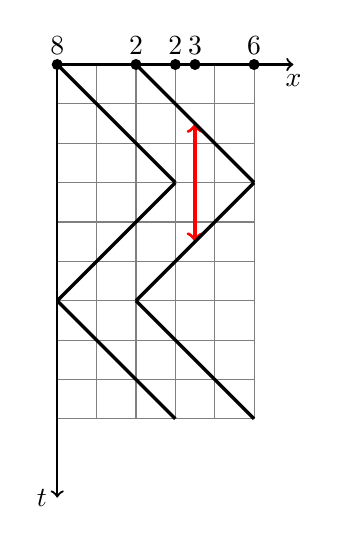
\begin{tikzpicture}
            \draw [help lines,thin,step=5mm] (0,-4.5) grid (2.5,0);
            \draw[thick, ->] (0,0) -- (3,0) node [below] {$x$};
            \draw[thick, ->] (0,0) -- (0,-5.5) node [left] {$t$};

            \fill ( 0   , 0) coordinate (c1) circle (2pt) node [above] {8};
            \fill ( 1   , 0) coordinate (c2) circle (2pt) node [above] {2};
            \fill ( 1.5 , 0) coordinate (c3) circle (2pt) node [above] {2};
            \fill ( 1.75, 0) coordinate (c4) circle (2pt) node [above] {3};
            \fill ( 2.5 , 0) coordinate (c5) circle (2pt) node [above] {6};

            \draw[very thick,red,<->] (1.75,-0.75)--(1.75,-2.25);

            \draw[very thick,-] ( 0  , 0  )--( 1.5,-1.5);
            \draw[very thick,-] ( 1.5,-1.5)--( 0  ,-3  );
            \draw[very thick,-] ( 0  ,-3  )--( 1.5,-4.5);
            \draw[very thick,-] ( 1  , 0  )--( 2.5,-1.5);
            \draw[very thick,-] ( 2.5,-1.5)--( 1  ,-3  );
            \draw[very thick,-] ( 1  ,-3  )--( 2.5,-4.5);
        \end{tikzpicture}
    \end{minipage}

    \begin{minipage}{0.5\hsize}
        \centering
        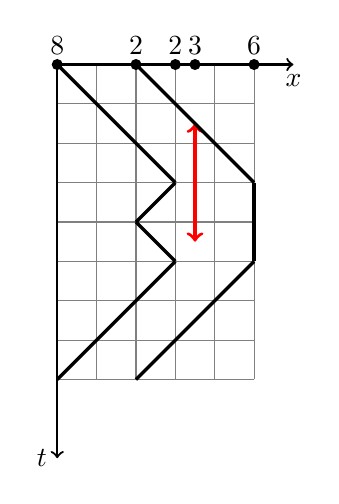
\begin{tikzpicture}
            \draw [help lines,thin,step=5mm] (0,-4) grid (2.5,0);
            \draw[thick, ->] (0,0) -- (3,0) node [below] {$x$};
            \draw[thick, ->] (0,0) -- (0,-5) node [left] {$t$};

            \fill ( 0   , 0) coordinate (c1) circle (2pt) node [above] {8};
            \fill ( 1   , 0) coordinate (c2) circle (2pt) node [above] {2};
            \fill ( 1.5 , 0) coordinate (c3) circle (2pt) node [above] {2};
            \fill ( 1.75, 0) coordinate (c4) circle (2pt) node [above] {3};
            \fill ( 2.5 , 0) coordinate (c5) circle (2pt) node [above] {6};

            \draw[very thick,red,<->] (1.75,-0.75)--(1.75,-2.25);

            \draw[very thick,-] ( 0  , 0  )--( 1.5,-1.5);
            \draw[very thick,-] ( 1.5,-1.5)--( 1  ,-2  );
            \draw[very thick,-] ( 1  ,-2  )--( 1.5,-2.5);
            \draw[very thick,-] ( 1.5,-2.5)--( 0  ,-4  );

            \draw[very thick,-] ( 1  , 0  )--( 2.5,-1.5);
            \draw[very thick,-] ( 2.5,-1.5)--( 2.5,-2.5);
            \draw[very thick,-] ( 2.5,-2.5)--( 1  ,-4  );
        \end{tikzpicture}
    \end{minipage}

    \end{tabular}
    \caption{巡査の協力が必要な例 \label{tikz:multiAgentExample2}}
    % 「可能な限り右に手伝いに行く」戦略が失敗する例
\end{figure}


\red{ここでは「間隔は厳密だが剰余の指定なし」に関する結果はないのだから、二段階に分けて説明する必要がないのでは。つまり、いきなり「間隔は厳密で、剰余の指定あり」の状況、あるいは更に定理2.4の状況に飛んだ方がすっきりするのでは。→}そこで我々は
{\timelimit}の代わりに「{\interval}」というものを考え,
各頂点を警備するにはその点の{\interval}ちょうどごとの時刻には訪問しなければならないという問題も考えた.
この「あえて短い間隔で訪問する」ことで得をしにくいような設定では,
さらに各頂点を訪問しなければならない最初の時刻も指定されるならば,
「できる限り右の方へ動く戦略」で
Lineの全点警備可能性を判定するができることを示した.
実際にはより一般的に,
Line上の訪問しなければならない座標と時刻のペアが有限個指定されている場合について
全点警備可能性判定問題を解くことができる.



\begin{theo}
    \label{theo:LineExactFinite}
    グラフの形状がLineで,
    各頂点$x_i$に対し訪問しなければならない時刻
    $t_{i,1}, t_{i,2}, \ldots, t_{i,{N_i}}$が指定されているとき,
    \red{$(t,x)$の集合?}
    「できる限り右の方へ動く戦略」で巡査を左側から1人ずつ割り当てることで
    全点警備可能性判定問題を解くことができる.
\end{theo}


「できる限り右の方へ動く戦略」は,次のように定義する.

% 定義
まず,図\ref{tikz:defLR}のように$t$-$x$平面の点$a = (t_a,x_a)$に対して領域$L(a), R(a)$を
\begin{align*}
    R(a) &:= \mathsetmid{(t,x)}{ -x + x_a + t_a < t < x - x_a + t_a } \\
    L(a) &:= \mathsetmid{(t,x)}{ (t,x) \not\in R(a) }
\end{align*}
と定義する.
$R(a),L(a)$を$R(t_a,x_a),L(t_a,x_a)$のようにも書くことにする.

\begin{figure}[h]
    \centering
    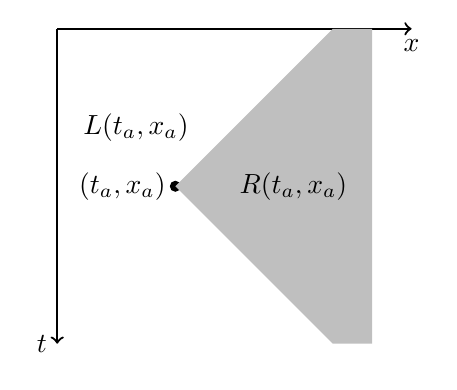
\begin{tikzpicture}
        % \draw [help lines, thin,step=10mm] (0,-5.5) grid (5.5,0);
        \draw[thick, ->] (0,0) -- (4.5, 0) node [below] {$x$};
        \draw[thick, ->] (0,0) -- (0,-4) node [left] {$t$};

        \fill ( 1.5,-2) coordinate (a) circle (2pt) node [left] {$(t_a,x_a)$};

        \fill [fill=lightgray]
            (a)--(3.5,0)--(4,0)--(4,-4)--(3.5,-4)--(a);

        \node (L) at (1,-1.25) {$L(t_a,x_a)$};
        \node (R) at (3,-2) {$R(t_a,x_a)$};
    \end{tikzpicture}
    \caption{$L(t_a,x_a)$ と $R(t_a,x_a)$ の定義 \label{tikz:defLR}}
\end{figure}



$t$-$x$平面上の点の集合$X'$が与えられたとき,
$X'$のどの点$a$に対する右側の三角形の領域$R(a)$にも含まれない領域
$\dbigcap_{a \in X'} L(a)$の(右の)境界線が軌跡であるような動き方を「できる限り右の方へ動く戦略」と定義する.
%
定理\ref{theo:LineExactFinite}は,
与えられた巡査のうち一番左を動く巡査$s_1$が(初期順序を保つ動き方において)どのような動き方をしたとしても
「できる限り右の方へ動く戦略」で$s_1$が訪問する点の一部しか訪問できないという意味で
「できる限り右の方へ動く戦略」は$s_1$の最適な動き方であり,
この動き方で1人ずつ巡査の動きを左側から定めることができるので巡査の必要最小数が分かるという主張である.

\red{ここを編集中}



\begin{proof}[証明\red{←何の?}]
全頂点を警備する任意の順序保存運行$A$で一番左側を動く巡査$s_1$の軌跡を考える.
%
もし$t$-$x$平面上のある点$(t_a,x_a)$から定まる$R(t_a,x_a)$に含まれる点$(t_b,x_b)$を
$s_1$の軌跡が通っているとすると,
$s_1$は$|x_a - x_b| > |t_a - t_b|$より時刻$t_a$に座標$x_a$を訪問できないので
$s_1$が一番左側を動くことから$(t_a,x_a)$が訪問されない点となってしまい矛盾する.
%
よって,$A$で一番左側を動く巡査$s_1$の軌跡は$\dbigcap_{a \in X'} L(a)$に含まれる.
$L(X') := \dbigcap_{a \in X'} L(a)$とする.

一方,この領域$L(X')$の境界線は傾き$1$または$-1$の線分のつながったものであるので,
$s_1$はこの境界線が軌跡となるように動くことができ,
そのようにすることで$L(X')$に含まれるすべての点を訪問でき
$A$での$s_1$の動きを改善できる.
%
$s_2, s_3, \ldots, s_m$の動き方も$X'$ の残りの点に対して
$s_1$のときと同様に決めていくことで$A$での動きを改善できる.

\red{ここを編集中}

\end{proof}

